\section{System Components}
\subsection{Frontend Components}
\subsection{Backend Components}
\subsection{Dataflow Diagram}
\begin{figure}[htbp]
  \begin{center}
    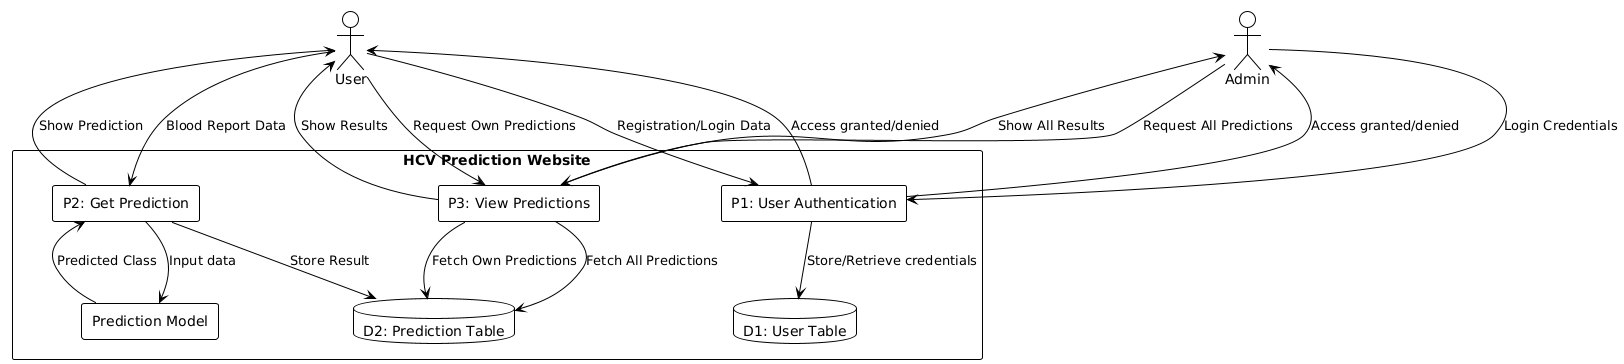
\includegraphics[width=\textwidth]{figures/dataflow.png}
  \end{center}
  \caption{Dataflow diagram of the website}\label{fig:dataflow}
\end{figure}

\subsection{User Interaction Diagram}

\begin{figure}[htbp]
  \begin{center}
    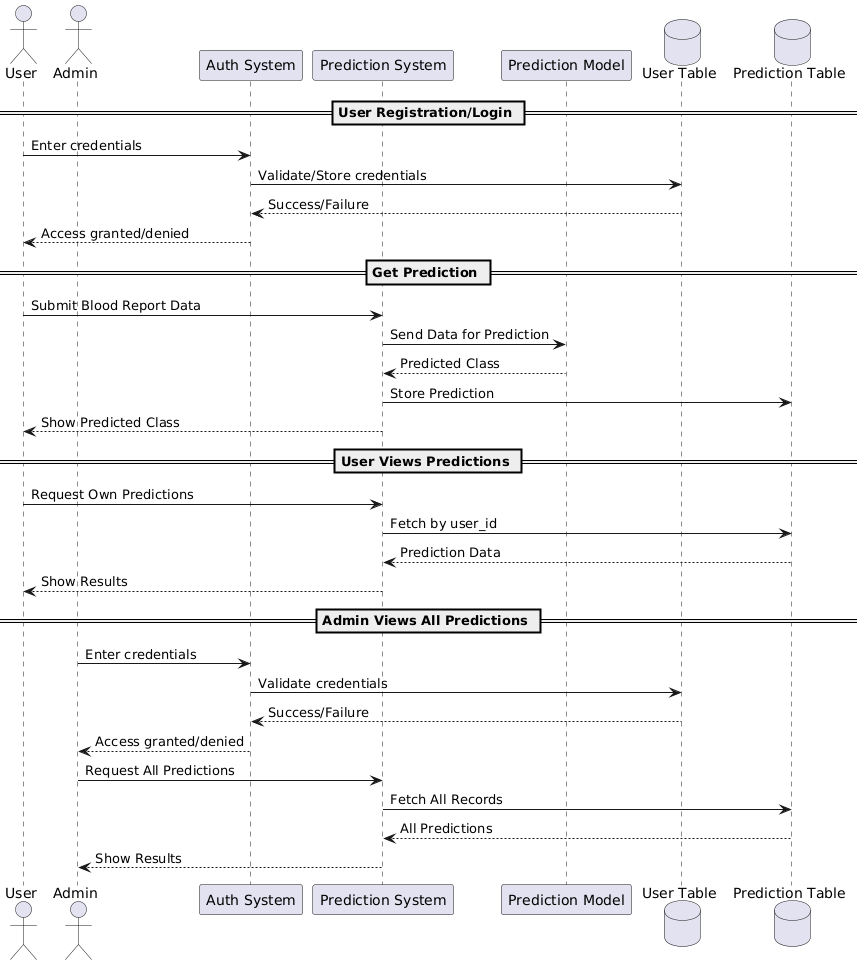
\includegraphics[width=\textwidth]{figures/sequence-diagram.png}
  \end{center}
  \caption{Sequence diagram for showing how the user interacts with the website}\label{fig:sequence-diagram}
\end{figure}

\subsection{Key Features}

\begin{figure}[htbp]
  \begin{subfigure}{0.5\textwidth}
    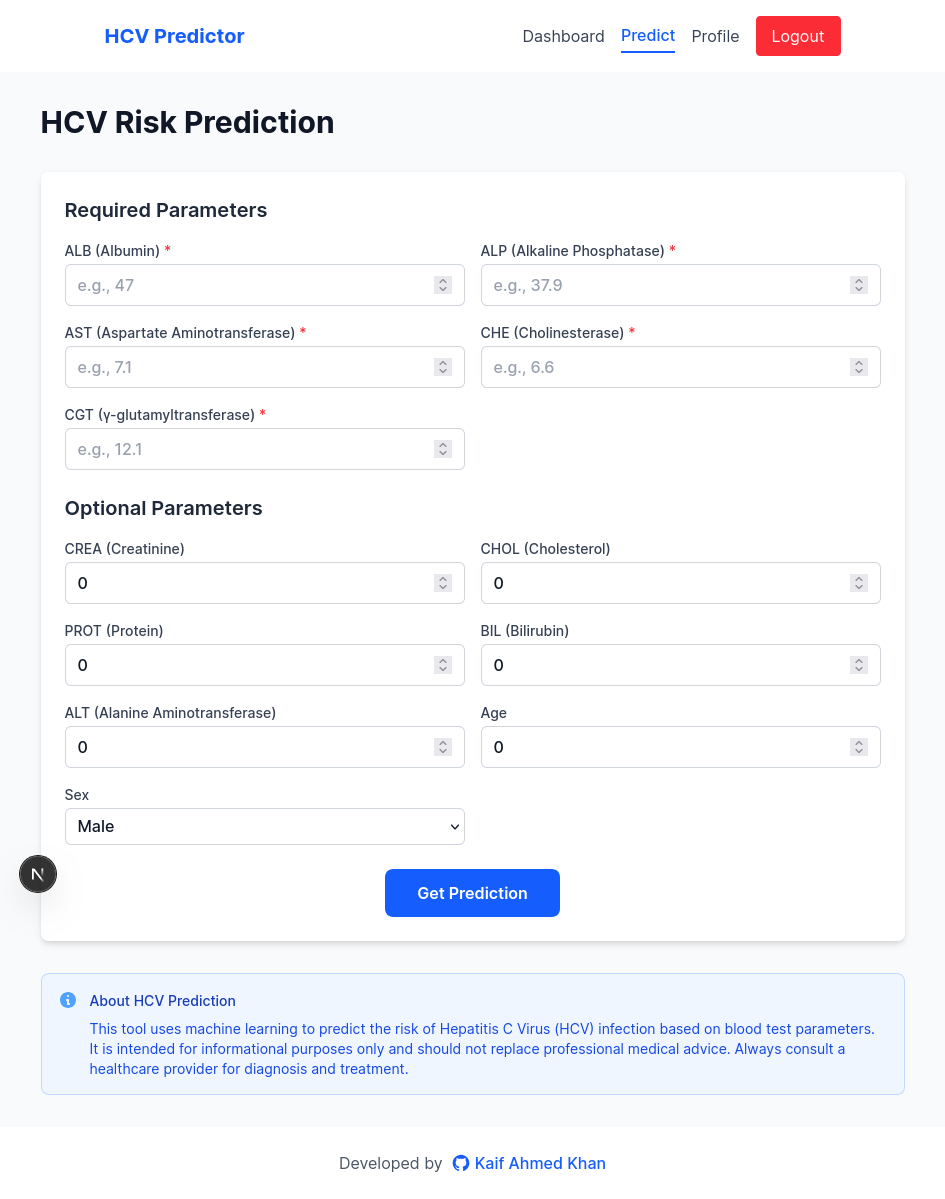
\includegraphics[width=0.9\linewidth, height=8cm]{figures/site/predict.png} 
    \caption{Prediction Page}
    \label{fig:subim1}
  \end{subfigure}
  \begin{subfigure}{0.5\textwidth}
    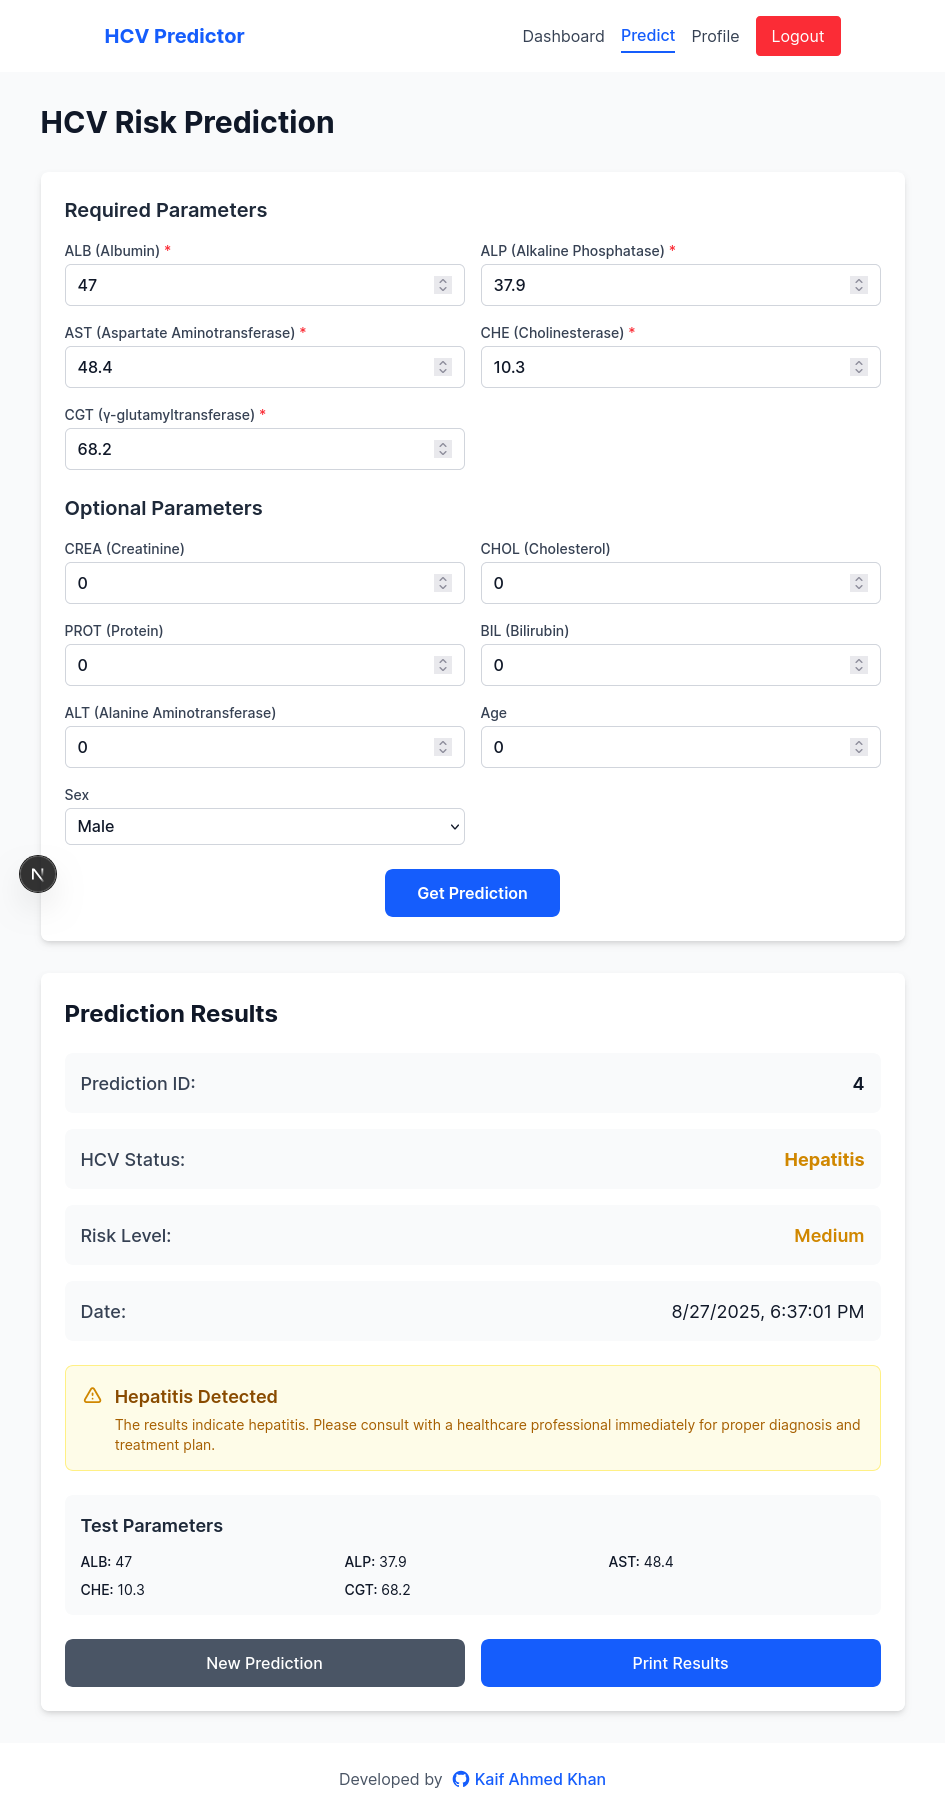
\includegraphics[width=0.9\linewidth, height=8cm]{figures/site/prediction02.png}
    \caption{Showing prediction result}
    \label{fig:predict}
  \end{subfigure}
  \begin{subfigure}{0.5\textwidth}
    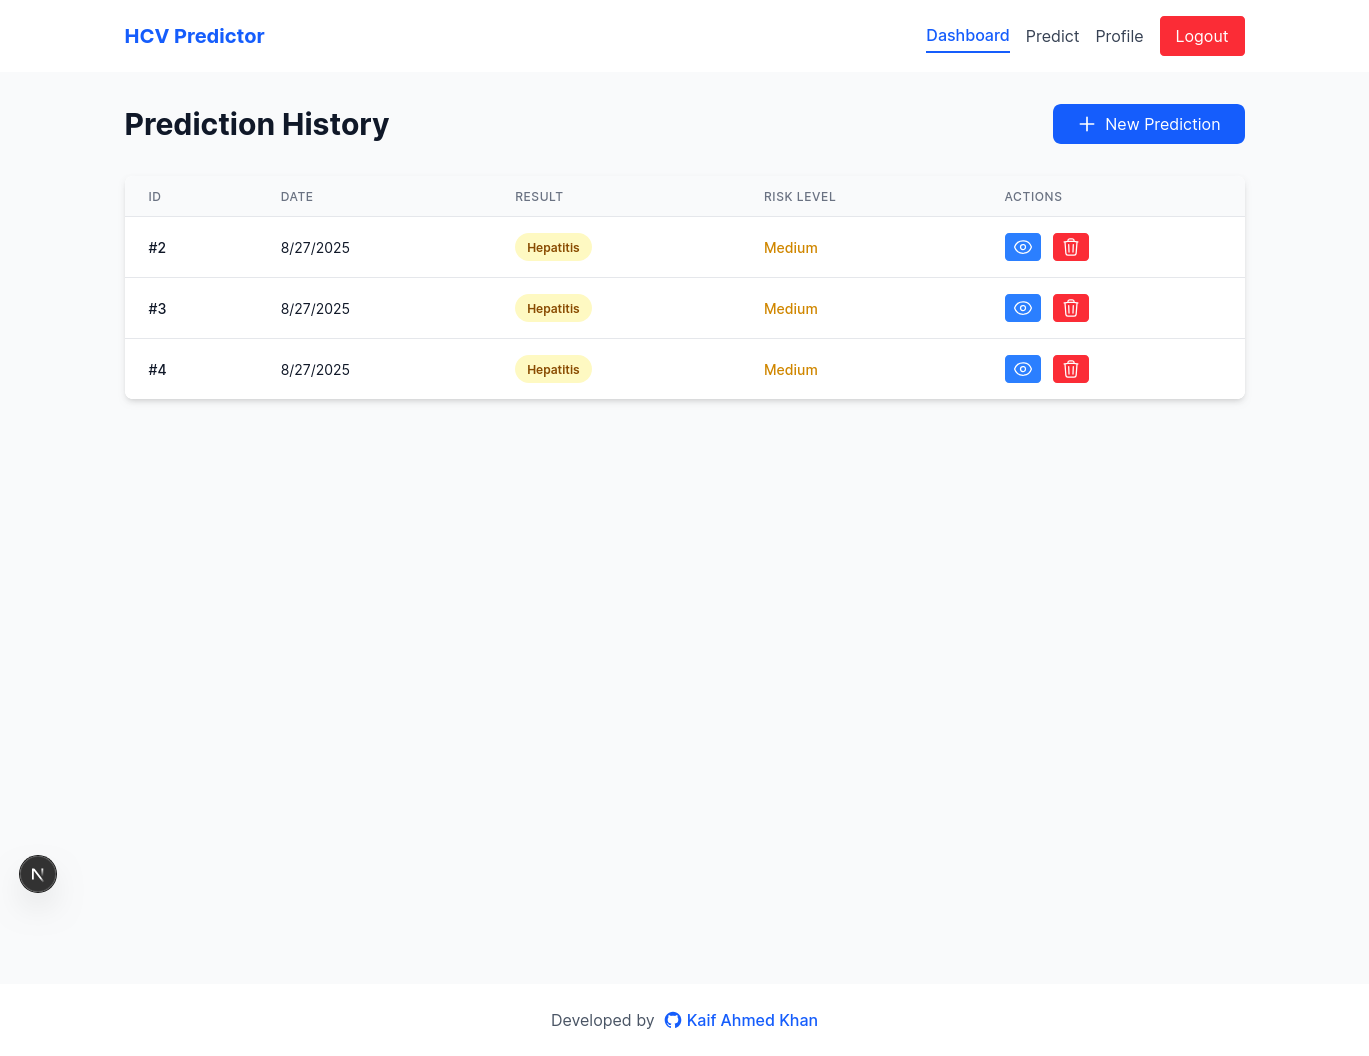
\includegraphics[width=0.9\linewidth, height=8cm]{figures/site/dashboard.png}
    \caption{Prediction history in dashboard}
    \label{fig:dashboard}
  \end{subfigure}
  \begin{subfigure}{0.5\textwidth}
    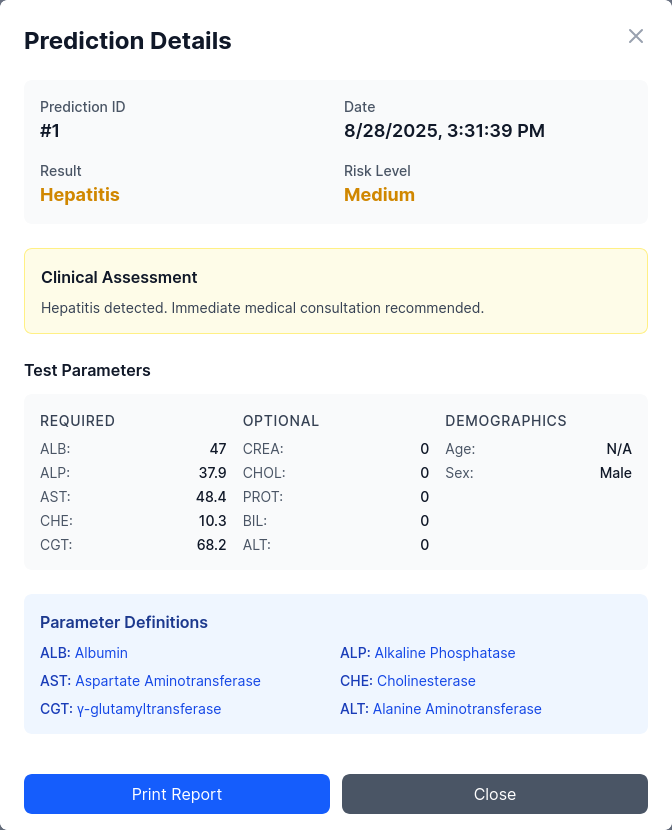
\includegraphics[width=0.9\linewidth, height=8cm]{figures/site/details.png}
    \caption{Prediction details modal}
    \label{fig:details}
  \end{subfigure}
  \caption{Prediction system and prediction history in dashboard}
  \label{fig:image2}
\end{figure}


\begin{figure}[htbp]
  \begin{subfigure}{0.5\textwidth}
    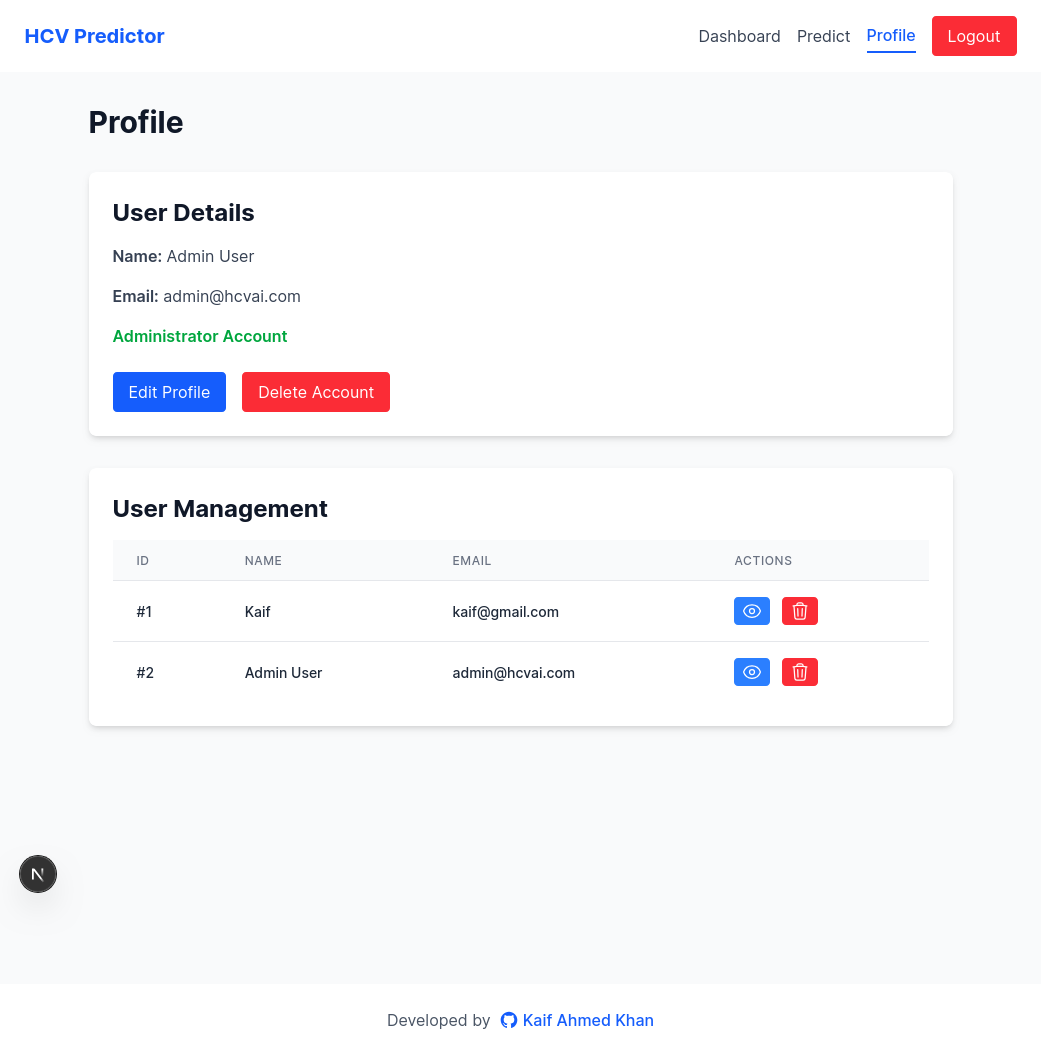
\includegraphics[width=0.9\linewidth, height=8cm]{figures/site/admin-profile.png} 
    \caption{Admin profile page}
    \label{fig:profile}
  \end{subfigure}
  \begin{subfigure}{0.5\textwidth}
    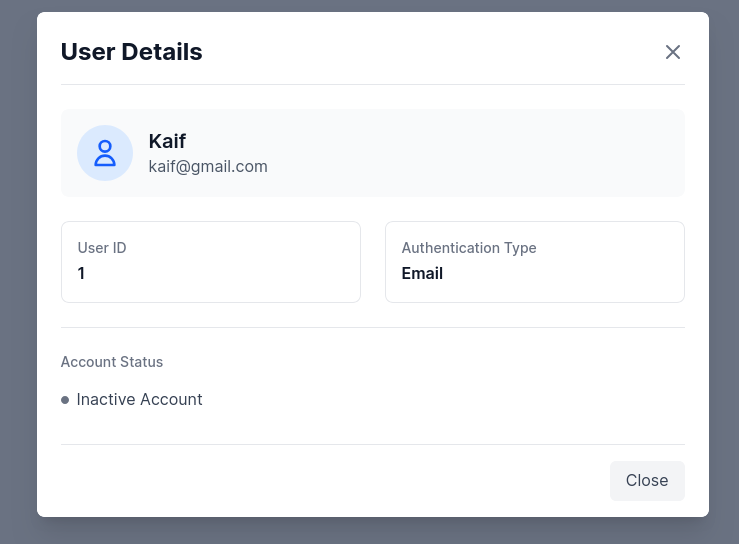
\includegraphics[width=0.9\linewidth, height=6cm]{figures/site/user-details.png}
    \caption{User details modal}
    \label{fig:userdetails}
  \end{subfigure}
  \begin{subfigure}{0.5\textwidth}
    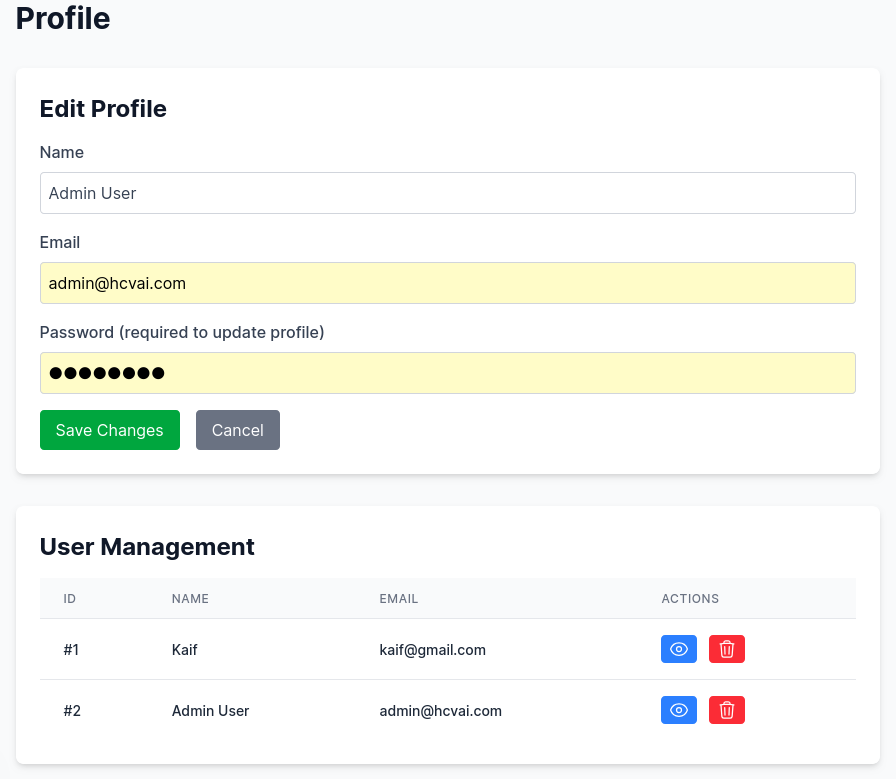
\includegraphics[width=0.9\linewidth, height=6cm]{figures/site/edit-profile.png}
    \caption{Edit profile details}
    \label{fig:edit}
  \end{subfigure}
  \begin{subfigure}{0.5\textwidth}
    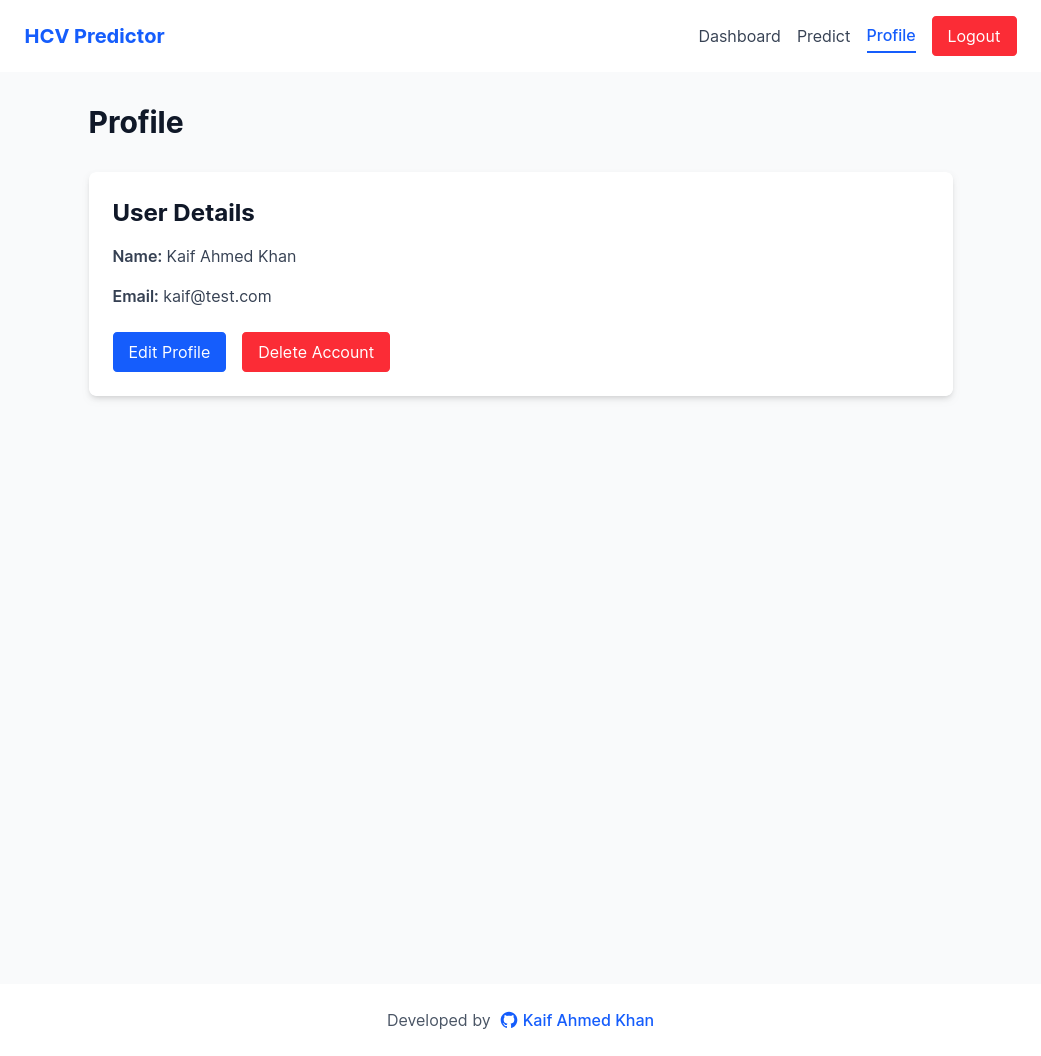
\includegraphics[width=0.9\linewidth, height=8cm]{figures/site/normaluser.png}
    \caption{Non-admin profile page}
    \label{fig:detail}
  \end{subfigure}
  \caption{User Management}
  \label{fig:image3}
\end{figure}

\subsection*{User Management}
\begin{itemize}
    \item User registration and login system with PostgreSQL database authentication.
    \item Role-based access control: Patients (users) and Admins.
    \item Secure storage of user information.
\end{itemize}
\subsection*{Prediction System}
\begin{itemize}
    \item Input form for blood report data (patient submits laboratory values).
    \item Pretrained machine learning model processes the input.
    \item Prediction of HCV stage (4 classes: 0--3).
    \item Prediction result is displayed instantly to the user.
\end{itemize}

\subsection*{Prediction History}
\begin{itemize}
    \item Patients can view their own previous predictions.
    \item Admins can view all users' predictions for monitoring and analysis.
\end{itemize}

\subsection*{Database Integration}
\begin{itemize}
    \item PostgreSQL database with two main tables:
    \begin{itemize}
        \item \textbf{User Table}: Stores user credentials and profile information.
        \item \textbf{Prediction Table}: Stores patient input, prediction results, and timestamps.
    \end{itemize}
\end{itemize}

\subsection*{Security and Roles}
\begin{itemize}
    \item Authentication system for both patients and admins.
    \item Role-specific permissions (patients see only their own data, admins see all data).
\end{itemize}

